\chapter{Methods}\label{ch:methods}
This chapter introduces the different methods used to quantify uncertainty for curved surfaces from partial point clouds without any extra information available. The task can be formulated for two different scenarios regarding the availability of additional data or prior information related to the 3D shape. In case of prior knowledge or additional data being unavailable, only the point cloud collected from multiple scans of the object can be used. Then our task can be defined as:
\begin{problemnotitle}{SingleCloud}{}
    \probleminput{A point cloud with $N_C$ points represented by $\mathbf{X}=\left\{\mathbf{x}_{i} \in \mathbb{R}^{3}\right\}_{i=1}^{N_C}$.}
    \problemoutput{A probabilistic estimate of the distance from the surface or probability of lying on the surface for any point $\mathbf{x} \in \mathbb{R}^{3}$.}
\end{problemnotitle}
\newline

On the other hand, if it is assumed that the kind of object the 3D shape belongs to is known, an additional dataset of related 3D shapes with partial and complete point clouds can be used. Then for a dataset of partial point clouds $\mathbf{X_P} \in \mathbb{R}^{N \times N_P \times 3}$ with $N$ instances of $N_P$ points in each incomplete point cloud instance, a corresponding dataset of complete point clouds $\mathbf{X_C} \in \mathbb{R}^{N \times N_C \times 3}$ with $N$ instances of $N_C$ points in each ground truth complete point cloud instance is available. Then the problem statement becomes:
\begin{problemnotitle}{DataCloud}{}
    \probleminput{A partial point cloud with $N_P$ points represented by $\mathbf{X}=\left\{\mathbf{x}_{i} \in \mathbb{R}^{3}\right\}_{i=1}^{N_P}$.}
    \problemoutput{A probabilistic estimate of the distance from the surface or probability of lying on the surface for any point $\mathbf{x} \in \mathbb{R}^{3}$.}
\end{problemnotitle}
\newline

Then the learned distribution over the distance field or the probabilistic surface reconstruction can be used for further downstream tasks.


\section{Empirical Uncertainty Quantification for Point Cloud Completion}\label{euqpcc}
In this section, a solution to the Problem~\ref{DataCloud} is proposed utilizing a point cloud completion method for the given input partial cloud. Instead of directly computing the probabilistic estimate of the underlying surface, multiple possible completions are generated from the input and then the surface along with the associated uncertainty is empirically estimated by matching points between generated complete clouds. The partial cloud is denoted by $\tilde{X}=\left\{\mathbf{\tilde{x}}_{i} \in \mathbb{R}^{3}\right\}_{i=1}^{N_P}$ and the generated complete cloud by $\hat{X}=\left\{\mathbf{\hat{x}}_{i} \in \mathbb{R}^{3}\right\}_{i=1}^{N_C}$. So the aim is to learn $p(\hat{X}|\tilde{X})$. During training, there is access to the ground truth complete cloud, which is denoted by $X=\left\{\mathbf{x}_{i} \in \mathbb{R}^{3}\right\}_{i=1}^{N_C}$. Since for any partial cloud, there are many possible complete clouds consistent with the partial cloud, one needs to learn to generate non-deterministic predictions depending upon some source of randomness. In Chapter~\ref{ch:background}, different ways to quantify uncertainty in deep learning models were reviewed, which provided an idea about how similar methods can also be implemented to generate different predictions with randomness. But first, the standard architecture used for point completion should be described.


    \subsection{General Structure of Point Completion Network}
    \begin{figure}[htb]
      \begin{center}
      \includegraphics[width=\linewidth]{figures/general_network.png}
      \end{center}
      \caption{General structure of network used for training point cloud completion. During training, ground truth complete cloud $X$ is input to the encoder E to output the encoding $\mathbf{y}$. Parallelly partial cloud $\tilde{X}$ is input to the encoder E to generate the encoding $\mathbf{\tilde{y}}$, which is then given to generator G outputting new encoding $\mathbf{\hat{y}}$ which is compared to $\mathbf{y}$. The decoder D, on the other hand, produces a complete cloud $\hat{X}$ from  $\mathbf{\hat{y}}$.}\label{fig:gen_net}
    \end{figure}
    The general structure of the network used for point cloud completion consists of an auto-encoder (encoder-decoder network) and a generator network. The encoder is denoted by E, the decoder by D, and the generator by G (see Figure~\ref{fig:gen_net}). Through the auto-encoder network's encoder, one can encode the partial shape represented by $\tilde{X}$ and the complete shape represented by $X$ to obtain the encodings $\mathbf{\tilde{y}}$ and $\mathbf{y}$, respectively. 
    \\
    Meanwhile, generator G generates a new encoding $\mathbf{\hat{y}}$ from the partial shape encoding $\mathbf{\tilde{y}}$ from which the decoder can produce a new complete shape $\hat{X}$. Generator G plays the role of the network that incorporates the randomness of the completion method, as it enables the generation of different encodings from the partial cloud encoding through G. Then, different complete clouds can be produced via the decoder, and the uncertainty of our completion method can be empirically estimated from the generated clouds. In the following section, the implementation details of the above idea is described.

    
    \subsection{Uncertainty in Encoding Generation}
        \subsubsection{MC Dropout or DropConnect in Generator}
        \begin{figure}[htb]
          \begin{center}
          \includegraphics[width=\linewidth]{figures/drop_network.png}
          \end{center}
      \caption{Network for point cloud completion uncertainty quantification using dropout or DropConnect. During inference, the original generator network is modified based on some masking ($\{m_i\}_{i=1}^M$) multiple times to produce different generators.}\label{fig:drop_net}
        \end{figure}
        One simple idea to generate different encodings via the generator is to use dropout or DropConnect in the generator network while training. As explained in section~\ref{MCDrop}, dropout or DropConnect can also be used during inference to generate different encodings and complete shapes corresponding to those encodings for a particular input partial cloud (see Figure~\ref{fig:drop_net}). 
        
        \subsubsection{Deep Ensemble of Generators}
        \begin{figure}[htb]
          \begin{center}
          \includegraphics[width=\linewidth]{figures/ensemble_network.png}
          \end{center}
          \caption{Network for point cloud completion uncertainty quantification using deep ensemble. Different generators (based on the ensemble construction strategy) are trained. During inference, different generators produce different encodings.}\label{fig:ens_net}
        \end{figure}
        An ensemble of generators can be used to train the point completion network. As described in section~\ref{Deepsemble}, there are many ways to construct the ensemble of generators. Different initializations of parameters were used in this work to create the ensemble. During inference, each generator in the ensemble outputs a different encoding, giving us different complete shapes(see Figure~\ref{fig:ens_net}).

        \subsubsection{Conditional Implicit Generative Model}
        \begin{figure}[htb]
          \begin{center}
          \includegraphics[width=\linewidth]{figures/implicit_gen_network.png}
          \end{center}
          \caption{Network for point cloud completion uncertainty quantification using conditional implicit generation. During inference, noise is sampled from a standard Gaussian distribution multiple times, and encodings are generated based on the different noises.}\label{fig:implicit_net}
        \end{figure}
        Another possible method to generate non-deterministic predictions from an input is to add random noise to the input before passing it to the generator. Eq.~\ref{IGM} can be reformulated for conditional implicit generative models as:
        \begin{equation}\label{IGM}
            \mathbf{\tilde{z}} \sim q(\mathbf{z}), \quad \mathbf{\hat{y}} =  \mathcal{G}_\theta(\mathbf{\tilde{z}}; \mathbf{\tilde{y}})
        \end{equation}
        where $\mathcal{G}$ is specified by an NN with parameters $\theta$. With different $\mathbf{\tilde{z}}$ different $\mathbf{\hat{y}}$ corresponding to different complete shape for a fixed $\mathbf{\tilde{y}}$ can be generated (see Figure~\ref{fig:implicit_net}).

    \subsection{Training Procedure}
        \subsubsection{Learning encoding for point clouds}
        \begin{figure}[htb]
          \begin{center}
          \includegraphics[width=\linewidth]{figures/emd_ae.png}
          \end{center}
          \caption{Training autoencoder by minimizing Earth mover's distance.}\label{fig:emd_ae}
        \end{figure}
        One can learn to produce the encoding of a given point cloud by training an autoencoder, which encodes the given input to a lower-dimensional feature vector called a latent code or an encoding, and subsequently decodes the encoding to reconstruct the original input. The autoencoder can be a standard autoencoder (AE), a variational autoencoder (VAE), or a vector-quantized variational autoencoder (VQ-VAE), depending on a deliberate choice. The autoencoder is trained for a reconstruction task on a point cloud dataset for both partial and complete shapes.
        \newline
        
        For instances of ground truth point cloud $X=\left\{\mathbf{x}_{i} \in \mathbb{R}^{3}\right\}_{i=1}^{N_C}$ from the dataset of complete clouds $\mathbf{X_C} \in \mathbb{R}^{N \times N_C \times 3}$, an encoder-decoder network is trained to learn an encoder mapping $\mathcal{E}: \mathbb{R}^{N_C \times 3} \rightarrow \mathbb{R}^{\ell}$ that takes the concatenation of coordinates of the $N_C$ points in complete cloud as input and produces an encoding in the latent space with dimension $\ell$ along with a decoder mapping $\mathcal{D}: \mathbb{R}^{\ell} \rightarrow \mathbb{R}^{N_C \times 3}$ that inverts the encoding back to a reconstructed point cloud with $N_C$ points as before. The autoencoder is trained using a reconstruction loss based on Earth Mover's Distance (EMD). The reconstruction loss for a point cloud $X$ is denoted as:
        \begin{equation}\label{emd_loss}
            L_{EMD} = d_{EMD}\left(X, \mathcal{D}(\mathcal{E}(X))\right),
        \end{equation}
        where $d_{EMD}\left(X, \mathcal{D}(\mathcal{E}(X))\right)$ denotes the Earth Mover's Distance between the input cloud and the reconstructed cloud (see Figure~\ref{fig:emd_ae}). Then the objective function for training the autoencoder can be computed as:
        \begin{equation}\label{emd_obj}
            \mathcal{L}_{EMD} = \mathbb{E}_{X \sim p(X)} \left[d_{EMD}\left(X, \mathcal{D}(\mathcal{E}(X))\right)\right]
        \end{equation}
        where $p(X)$ denotes a distribution over the space of complete clouds from which we sample.
        \newline
        
        The encoding produced by the encoder provides a ready-made representation, which implicitly captures the shape manifold for a point cloud, to be used in downstream tasks. So, once training is done, the network parameters are fixed while using the encoder and decoder in any subsequent network. As for the instances of point cloud $\tilde{X}=\left\{\mathbf{\tilde{x}}_{i} \in \mathbb{R}^{3}\right\}_{i=1}^{N_P}$ from the dataset of partial clouds $\mathbf{X_P} \in \mathbb{R}^{N \times N_P \times 3}$, a separate auto-encoder is not trained. Rather, the partial cloud is directly passed to the autoencoder trained with complete clouds to produce encoding in the latent space, which is known to work better for downstream applications. To do that, some points from the partial point cloud can be copied to match the number of points in the complete cloud before feeding it to the encoder. Alternatively, an encoder invariant of point set size, similar to PointNet~\cite{PointNet}, can be used.


        \subsubsection{Learning to generate multiple point clouds}
        \begin{figure}[htb]
          \begin{center}
          \includegraphics[width=\linewidth]{figures/implicit_gen_network_imle.png}
          \end{center}
          \caption{Training network for point cloud completion uncertainty quantification using conditional implicit maximum likelihood estimation. During training, not all encodings generated from G are compared with the complete cloud encoding $\mathbf{y}$. Only the closest encoding is selected during training.}\label{fig:imle}
        \end{figure}
        Training differs according to the method selected for uncertainty quantification (more precisely, methods for inducing randomness) to produce different complete shapes. If dropout or DropConnect is used, the training procedure becomes quite straightforward. The same general structure for point completion depicted in Figure~\ref{fig:gen_net} is followed with the generator $G$ using dropout or DropConnect during training. If an ensemble of generators with $M$ models is used, then each generator needs to be trained individually, resulting in $M$ different training sequences similar to the procedure shown in Figure~\ref{fig:ens_net}. In this case, the inference and training follow the same pattern. 
        \newline
        
        Finally, for the implicit generation, one learns to produce different complete shapes for a fixed partial input based on the noise injected into the generator. Since only one possible target shape is available for each partial shape, it needs to be trained differently from just computing the loss based on the one-to-one correspondence. Otherwise, any addition of noise will be rendered inconsequential, resulting in mode collapse and similar completion results. Note that this is not an issue for dropout or ensemble models. With dropping out, the uncertainty is inherently induced through the different selection of weights or nodes during training. For the ensemble, all the models are trained separately. 
        \\
        For training conditional implicit generative models, conditional Generative Adversarial Networks (GANs) had been the go-to approach for a long period. However, due to several drawbacks, such as mode collapse, the popularity of GANs has dwindled, with new approaches overturning the downsides of using GANs. One such method, called Implicit Maximum Likelihood Estimation (IMLE), was introduced by~\cite{IMLE}.~\cite{PCCIMLE} already applied the same idea for point cloud completion, which is adopted here. The authors of~\cite{PCCIMLE} demonstrated that using conditional IMLE to train implicit generation yields more diverse completion results, thereby resolving the mode collapse issue. Here, rather than comparing all the generated encodings ($\{\mathbf{\hat{y}}_i\}_{i=1}^M$) with the encoding of the complete shape $\mathbf{y}$, only the one closest to $\mathbf{y}$ is chosen as shown in Figure~\ref{fig:imle}. This way, not every generated encoding is close to the encoding of the complete cloud, but every complete shape encoding has one generated encoding trained to be close in the latent space. This ensures that mode collapse does not happen, and every complete shape in the training data has at least one similar shape generated.

        \begin{figure}[htb]
          \begin{center}
          \includegraphics[width=\linewidth]{figures/losses_main_network.png}
          \end{center}
          \caption{Losses for training the main network for point cloud completion with uncertainty.}\label{fig:losses_main}
        \end{figure}
        To train the network (generator), the loss functions that are to be minimized need to be specified (see Figure~\ref{fig:losses_main}). As discussed above, the parameters of the encoder-decoder network trained for reconstruction are fixed. For a ground truth point cloud $X=\left\{\mathbf{x}_{i} \in \mathbb{R}^{3}\right\}_{i=1}^{N_C}$ from the dataset of complete clouds $\mathbf{X_C} \in \mathbb{R}^{N \times N_C \times 3}$, it is fed to the encoder network to get its encoding $\mathbf{y}$. Similarly, the corresponding point cloud $\tilde{X}=\left\{\mathbf{\tilde{x}}_{i} \in \mathbb{R}^{3}\right\}_{i=1}^{N_P}$ from the dataset of partial clouds $\mathbf{X_P} \in \mathbb{R}^{N \times N_P \times 3}$ is passed to the encoder to obtain its encoding $\mathbf{\tilde{y}}$. Now, $\mathbf{\tilde{y}}$ is passed through the generator according to the selected architecture among the ones explained above. For dropout or DropConnect, only one encoding $\mathbf{\hat{y}}$ is generated and compared with $\mathbf{y}$. Otherwise, $M$ encodings $\{\mathbf{\hat{y}}_i\}_{i=1}^M$ are generated corresponding to the $i$-th model in the ensemble or $i$-th noise sampled for implicit generation. In the ensemble method, each of $\{\mathbf{\hat{y}}_i\}_{i=1}^M$ is compared to $\mathbf{y}$. In implicit generation, the proposed IMLE method is followed, and the encoding in $\{\mathbf{\hat{y}}_i\}_{i=1}^M$ closest to $\mathbf{y}$ with $\mathbf{y}$ is compared. The corresponding loss function between two encodings is denoted as:
        \begin{equation}\label{latent_loss}
            L_{encoding}(\mathbf{y}, \mathbf{\hat{y}}) = \left\|\mathbf{y} - \mathbf{\hat{y}}\right\|_2^2,
        \end{equation}
        which is the Euclidean distance between the two encodings. 
        \\
        One also needs to ensure that the complete shapes generated are faithful to the partial shape. To maintain the fidelity of the completion results produced from the encodings output by the generator, the unidirectional Hausdorff distance between the partial cloud and the generated complete cloud is used. The corresponding loss is denoted as:
        \begin{equation}\label{fidelity_loss}
            L_{fidelity}(\tilde{X}, \hat{X}) = \max_{\mathbf{\tilde{x}}_{i} \in \tilde{X}} \min_{\mathbf{\hat{x}}_{j} \in \hat{X}} \left\|\mathbf{\tilde{x}}_{i}-\mathbf{\hat{x}}_{j}\right\|_2,
        \end{equation}
        where $\hat{X}=\left\{\mathbf{\hat{x}}_{j} \in \mathbb{R}^{3}\right\}_{j=1}^{N_C}$ is the set of generated point clouds. So the overall objective for training the network is:
        \begin{equation}\label{gen_obj}
            \begin{aligned}
                \mathcal{L}_{pcc} = \mathbb{E}_{X, \tilde{X} \sim p(X, \tilde{X})} \left[\lambda_{encoding} L_{encoding}\left(\mathcal{E}(X), \mathcal{G}_\theta(\mathcal{E}(\tilde{X}))\right)\right \\
                + \left\lambda_{fidelity} L_{fidelity}(\tilde{X}, \mathcal{D}\left(\mathcal{G}_\theta(\mathcal{E}(\tilde{X})))\right)\right]
            \end{aligned},
        \end{equation}
        where $\mathcal{E}$ is the encoder mapping, $\mathcal{D}$ is the decoder mapping, and $\mathcal{G}_\theta$ is the generator mapping by the NN parametrized by $\theta$. For IMLE, the above objective changes to:
        \begin{equation}\label{gen_obj_imle}
            \begin{aligned}
                \mathcal{L}_{pcc}^{imle} = \mathbb{E}_{X, \tilde{X} \sim p(X, \tilde{X}), \mathbf{Z}} \left[\lambda_{encoding} \min_{i=1, \ldots, M} L_{encoding}\left(\mathcal{E}(X), \mathcal{G}_\theta(\mathcal{E}(\tilde{X}), \mathbf{\tilde{z}}_i)\right)\right \\
                + \left\lambda_{fidelity} L_{fidelity}(\tilde{X}, \mathcal{D}\left(\mathcal{G}_\theta(\mathcal{E}(\tilde{X})))\right)\right]
            \end{aligned},
        \end{equation}
        where $\mathbf{Z} = (\mathbf{\tilde{z}}_1, \ldots, \mathbf{\tilde{z}}_M)^T$ such that $\mathbf{\tilde{z}}_i \sim \mathcal{N}(0, I_z) \forall i=\{1, \ldots, M\}$ with noise dimension $z$ and hyperparameter M.


    \subsection{Uncertainty Map Computation with Matching}
    \begin{figure}[htb]
      \begin{center}
      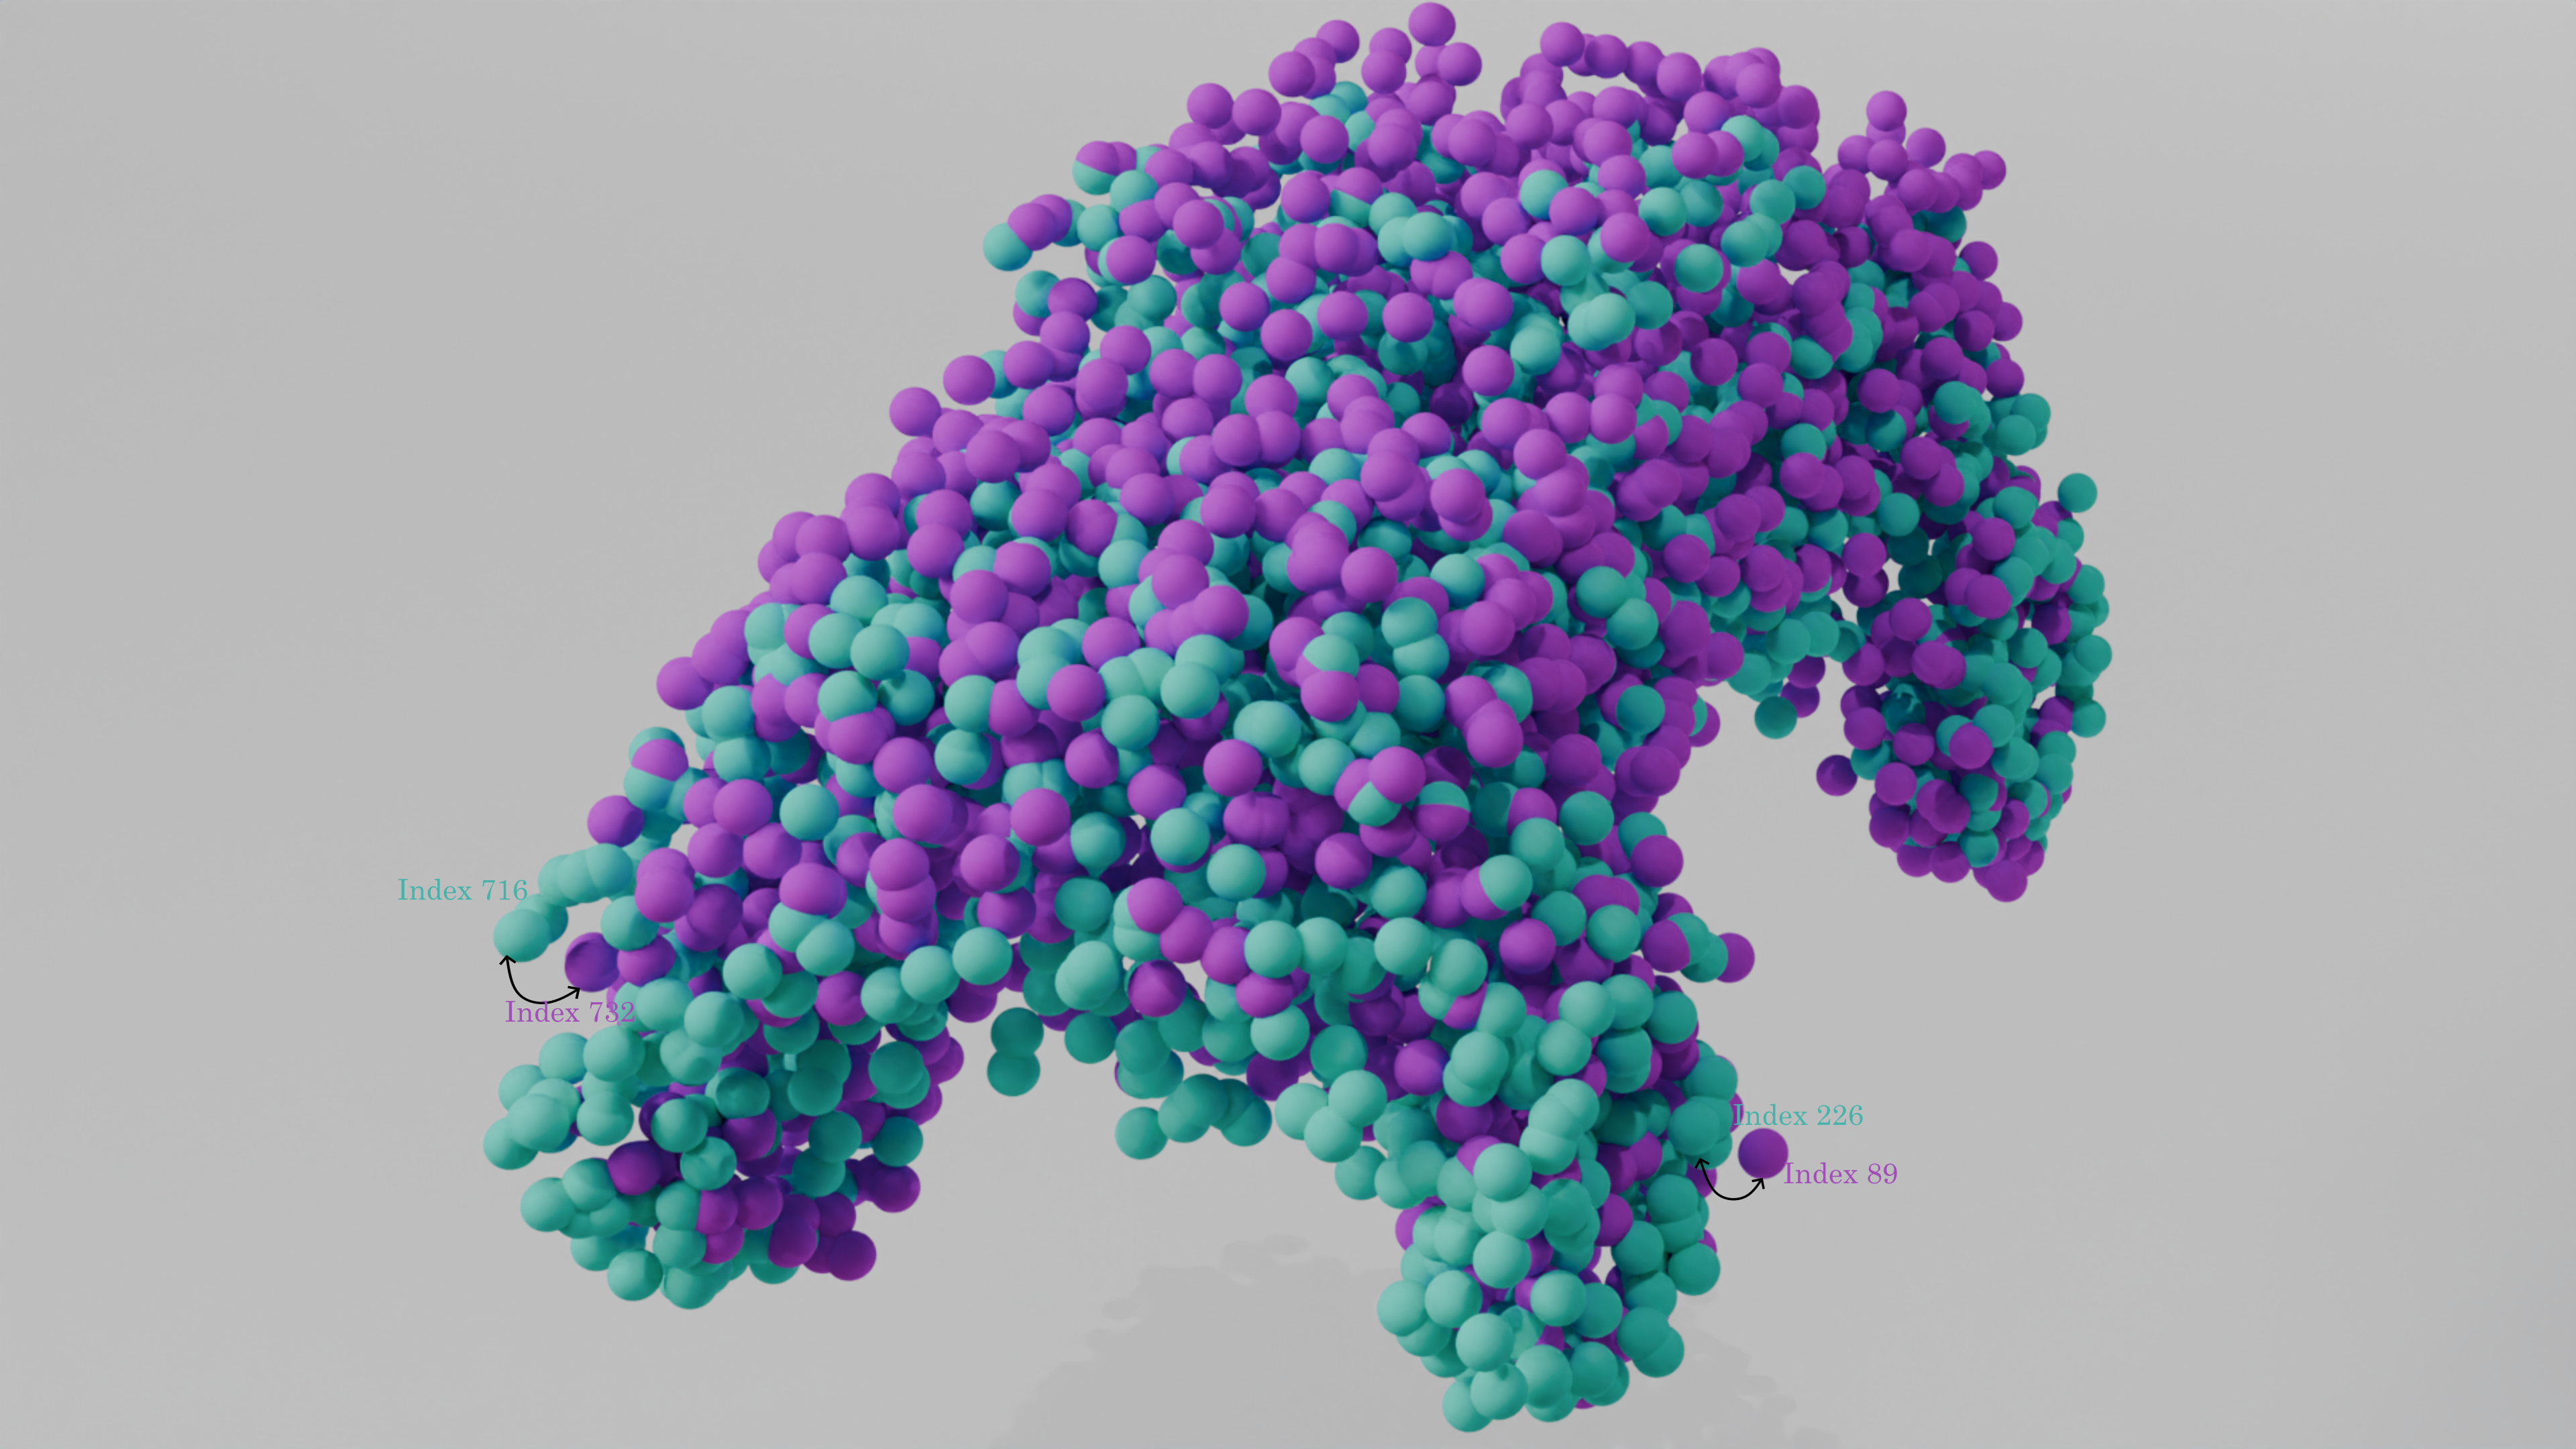
\includegraphics[width=\linewidth]{figures/matching_edited.png}
      \end{center}
      \caption{Linear assignment for matching between a pair of generated point clouds. For each point in the green cloud, the closest point in the purple cloud is located based on some cost function. Notice that the representative indices of the matched points are different in the respective tensors of the generated clouds.}\label{fig:matching}
    \end{figure}
    Rather than naively computing the index-wise mean and variance of the 3D coordinates of the generated complete clouds, the point sets can be matched between themselves as one-to-one mappings of points. Such matchings between two point clouds can be computed using a minimum-weight matching or linear assignment with an appropriate cost of matching a point from one cloud to a point in another. Hungarian matching algorithm~\cite{Hungarian} or a modified version of Jonker-Volgenant algorithm~\cite{RectAssign} were applied to perform the matching between clouds. Euclidean distance between points was used as the cost function. One of the generated complete clouds was selected at random, and one-to-one mappings with points in the remaining complete clouds were identified. The resulting matching was then used to compute the mean and variance estimations of the predicted complete point cloud.


\section{Empirical Uncertainty Quantification for Implicit Neural Representation}\label{euqinr}
In this section, a solution to the Problems~\ref{SingleCloud} and~\ref{DataCloud} is proposed by predicting uncertain implicit representations for the given input cloud. An implicit representation is a function $f: \mathbb{R}^{3} \mapsto \mathbb{R}$ such that the zero level set of $f$ precisely approximates the surface on the 3D shape denoted by $\mathcal{S}$ :
\begin{equation}
\mathcal{S} \approx \left\{\mathbf{x} \in \mathbb{R}^{3} \mid f(\mathbf{x})=0\right\}
\end{equation}
\newline

Instead of directly computing the probabilistic estimate of the underlying surface, one can first generate multiple possible implicit representations $\{f_i: \mathbb{R}^3 \mapsto \mathbb{R}\}_{i=1}^M$ from the input and then empirically estimate the surface along with the associated uncertainty from the different implicit representations. From previous works, it is known that the neural implicit function $f$ usually approximates the (un-)signed distance function (UDF/SDF), which maps any point in space to the distance to its closest point on the surface. For a function $f$ to be a distance function corresponding to a given point cloud $X=\left\{\mathbf{x}_{i} \in \mathbb{R}^{3}\right\}_{i=1}^{N_C}$, it needs to satisfy some conditions or constraints as enumerated below~\cite{DiGS, NeuralHessian}:
\begin{enumerate}
    \item Dirichlet condition or manifold constraint: the observed points in the point cloud lie on the surface of the object, $f(\mathbf{x})=0$ for $\mathbf{x} \in X$.
    \item Eikonal constraint: all points have a unit gradient, $\|\nabla f\|=1$.
    \item Neumann condition or normal constraint:  the gradients of points match the ground truth normal field if normal information is available, $\nabla f=\mathcal{N}$, where $\mathcal{N}$ is the normal field.
    \item Non-manifold constraint: non-manifold points (points not on the surface) have the same value as their ground truth SDF or UDF if the distance values are available.
    \item Non-manifold penalisation constraint: non-manifold points have non-zero implicit function values.
\end{enumerate}
Out of the above constraints, while the manifold constraint and one of the Eikonal constraint or the Non-manifold constraint are necessary, the rest are mostly used as additional criteria to enhance the results~\cite{DiGS}. Since only unoriented point clouds without normal information or SDF/UDF values are available for supervision, normal constraint and non-manifold constraint cannot be used. The remaining 3 constraints for a given point cloud $X=\left\{\mathbf{x}_{i} \in \mathbb{R}^{3}\right\}_{i=1}^{N_C}$ are used, which give rise to the following loss functions:
\begin{equation}\label{manifold_sdf}
    \mathcal{L}_{\text {manifold }}=\int_{X}\|f(x)\|_{1} d x \approx \frac{1}{N_C}\sum_{i=1}^{N_C}\|f(\mathbf{x}_i)\|_1
\end{equation}
\begin{equation}\label{non_manifold_sdf}
    \mathcal{L}_{\text {non-manifold }}=\int_{\underline{X}} \exp \left(-\alpha\|f(x)\|_{1}\right) d x \approx \frac{1}{N_C}\sum_{i=1}^{N_C} \exp \left(-\alpha\|f(\underline{\mathbf{x}_i})\|_1\right),
\end{equation}
where $\underline{X}=\left\{\underline{\mathbf{x}_i} \in \mathbb{R}^{3}\right\}_{i=1}^{N_C}$ is the set of points off the surface and $\alpha>>1$.
\begin{equation}\label{Eikonal}
     \begin{aligned}
         \mathcal{L}_{\text {Eikonal }}=\int_{X \cup \underline{X}} \| \| \nabla f(x)\left\|_{2}-1\right\|_{1} d x \\
         \approx \frac{1}{N_C}\sum_{i=1}^{N_C} \left(\| \| \nabla f(\mathbf{x}_i)\left\|_{2}-1\right\|_{1} + \| \| \nabla f(\underline{\mathbf{x}_i})\left\|_{2}-1\right\|_{1} \right).
     \end{aligned}
\end{equation}
The combined objective function can then be computed as:
\begin{equation}\label{inr_loss1}
    \mathcal{L}_{inr}= \lambda_{\text {manifold }} \mathcal{L}_{\text {manifold }}+\lambda_{\text {non-manifold }} \mathcal{L}_{\text {non-manifold }}+ \lambda_{\text {Eikonal }} \mathcal{L}_{\text {Eikonal }}
\end{equation}
where $\lambda_{\text {manifold }}, \lambda_{\text {non-manifold }}, \lambda_{\text {Eikonal }}$ are the corresponding regularization weights.
\newline

However, optimizing the above objective is not sufficient to produce optimal results, as demonstrated by~\cite{DiGS, NeuralHessian}. As discussed in section~\ref{INR-old}, several works have tried to solve this issue by introducing an additional loss depending upon the intended geometric effect. Since only unoriented point clouds are available as inputs, the loss based on the Hessian matrix defined in~\cite{NeuralHessian} was employed. The loss function associated with the Hessian matrix can be computed as:
\begin{equation}\label{Hessian1}
    \mathcal{L}_{\text{Hessian }} = \int_{\circled{$X$}} \left|Det(\mathbf{H}_f(x))\right| d x \approx \frac{1}{N_C}\sum_{i=1}^{N_C} \left|Det\left(\mathbf{H}_f\left(\circled{$\mathbf{x}_i$}\right)\right)\right|,
\end{equation}
where $\circled{$X$}=\left\{\circled{$\mathbf{x}_i$} \in \mathbb{R}^{3}\right\}_{i=1}^{N_C}$ is the set of points close to the surface and $Det(\cdot)$ refers to the determinant of the matrix. So the overall objective function now becomes:
\begin{equation}\label{Hessian2}
    \begin{aligned}
        \mathcal{L}_{inr}= \lambda_{\text {manifold }} \mathcal{L}_{\text {manifold }}+\lambda_{\text {non-manifold }} \mathcal{L}_{\text {non-manifold }}+ \lambda_{\text {Eikonal }} \mathcal{L}_{\text {Eikonal }}
        \\
        +\lambda_{\text{Hessian }} \tau \mathcal{L}_{\text{Hessian }},
    \end{aligned}
\end{equation}
where $\tau$ is the annealing factor defined in~\cite{NeuralHessian}. Now that the objective is defined, the method for introducing randomness in implicit function prediction to calculate uncertainty can be discussed.


    \subsection{Predicting Implicit Representation with Randomness}
    \begin{figure}[htb]
      \begin{center}
      \includegraphics[width=\linewidth]{figures/inr_network.png}
      \end{center}
      \caption{General structure of network used for training implicit function with randomness. During training, the partial cloud $\tilde{X}$ is input to the encoder E to output the encoding $\mathbf{\tilde{y}}$. Manifold, non-manifold, and near points conditioned on $\mathbf{\tilde{y}}$ and noises are fed to the decoder D$_{\text{INR}}$ to predict the implicit function corresponding to the noise.}\label{fig:inr_net}
    \end{figure}
    Randomness can be introduced into the network architecture that approximates the implicit function using any of the uncertainty quantification methods discussed in Section~\ref {back_uqdl}. For Problem~\ref{SingleCloud}, the network structure is straightforward. Existing shape space learning architectures for point clouds can be used, such as a standard or variational autoencoder, with the decoder output being the implicit representation instead of a reconstructed cloud. On the other hand, for Problem~\ref{DataCloud}, partial and complete cloud pairs are available during training, but only the partial cloud is available for inference. Therefore, an information disparity exists between the training and inference processes if the implicit representation is directly learned from complete clouds in the shape space. To gain a clearer understanding of the information lost without the complete cloud, the sampling procedure used to learn the implicit function is described first.
    \newline
    
    To sample points not on the surface (points in the set $\underline{X}$), a bounding box around the point cloud was found, and points within that box were sampled uniformly. Considering most points inside the box are off the surface, sampling a point on the surface is highly unlikely. To sample points close to the surface (points in the set \circled{$X$}), the sampling used in~\cite{IGR, SALD, NeuralHessian} was emulated. For each point $\mathbf{x}_i$ on the surface, the distance to the $k$-th nearest point ($k=50$ used by previous methods) was found and denoted as $d$. Then one point from the Gaussian distribution $\mathcal{N}(\mathbf{x}_i, d^2I)$ was sampled to find a point close to the surface. One can observe that while sampling of non-manifold points is not affected by the unavailability of a complete cloud, sampling of points close to the surface differs. So, using points close to the surface was avoided during inference. Additionally, since only the partial point cloud is available at test time, the encoding of the complete cloud cannot be used during learning. With all that in mind, the architecture depicted in Figure~\ref{fig:inr_net} is proposed.
    \newline
    
    The complete point cloud $X$ is considered as the points lying on the surface (manifold points). The non-manifold and near point sets $\underline{X}$ and \circled{$X$} were sampled as explained. The partial cloud $\tilde{X}$ is fed to the encoder E to get the encoding $\mathbf{\tilde{y}}$. Parallelly, multiple noises $\mathbf{Z} = (\mathbf{\tilde{z}}_1, \ldots, \mathbf{\tilde{z}}_M)^T$ were sampled such that $\mathbf{\tilde{z}}_i \sim \mathcal{N}(0, I_z) \forall i=\{1, \ldots, M\}$ with noise dimension $z$ and hyperparameter $M$. The manifold, non-manifold, and near points conditioned on the encoding $\mathbf{\tilde{y}}$ and noises are then passed to the decoder D$_{\text{INR}}$ to predict the implicit function corresponding to each noise. If, during training, the objective for the implicit function predicted for each noise is minimized, the issue of mode collapse might appear. This will lead to a lack of diversity in predicted implicit functions. Therefore, during training, only the noise leading to the implicit function with minimum manifold loss ($\mathcal{L}_{\text {manifold }}$) was chosen for computing the rest of the objective function and performing backpropagation. During inference, different implicit functions based on different noises were predicted, and the mean and variance at any point were empirically estimated based on these predicted functions to obtain our reconstructed surface with associated uncertainty.
    \newline
    
    The learned encoding also needs to be regularized for better shape space learning using autoencoder architectures. For a standard autoencoder, the regularization loss can be computed as:
    \begin{equation}\label{reg_latent}
        \mathcal{L}_{\text {reg }} = \left\|\mathcal{E}(\tilde{X})\right\|_2^2,
    \end{equation}
    where $\mathcal{E}$ is the encoder mapping. For a variational autoencoder, the  regularization loss can be computed as (similar to~\cite{SAL}):
    \begin{equation}\label{reg_latent}
        \mathcal{L}_{\text {reg }} = \left\|\mu\left(\mathcal{E}(\tilde{X})\right)\right\|_1 +\left\|diag(\Sigma\left(\mathcal{E}(\tilde{X})\right)\right\|_1,
    \end{equation}
    where $diag$ is the diagonal matrix, $\mu$ denotes the latent prediction (mean function) and $\Sigma$ refers to the covariance matrix for latent prediction. Such regularization enforces the latent means to be near zero and the covariances to be close to identity matrices. With the addition of the regularization term, the overall objective function becomes:
    \begin{equation}\label{Hessian3}
        \begin{aligned}
            \mathcal{L}_{inr}= \lambda_{\text {manifold }} \mathcal{L}_{\text {manifold }}+\lambda_{\text {non-manifold }} \mathcal{L}_{\text {non-manifold }}+ \lambda_{\text {Eikonal }} \mathcal{L}_{\text {Eikonal }}
            \\
            + \lambda_{\text{Hessian }} \tau \mathcal{L}_{\text{Hessian }} + \lambda_{\text {reg }} \mathcal{L}_{\text {reg }},
        \end{aligned}
    \end{equation}

    

\section{Gaussian Process-based Uncertainty Quantification for 3D Shapes}\label{gpuq}
In this section, the Problems~\ref{SingleCloud} and~\ref{DataCloud} are tackled by describing an uncertain implicit representation for the given input cloud by a Gaussian process. Several existing works (see section~\ref{Stoch-old}) follow a similar approach for a single point cloud (Problem~\ref{SingleCloud}). Therefore, the focus in this thesis will be solely on methods to solve Problem~\ref{DataCloud}.

\begin{figure}[htb]
      \begin{center}
      \includegraphics[width=\linewidth]{figures/gpr_network.png}
      \end{center}
      \caption{General structure of network used for learning feature mapping. During training, the partial cloud $\tilde{X}$ is input to the encoder E to output the encoding $\mathbf{\tilde{y}}$. Manifold and non-manifold points conditioned on $\mathbf{\tilde{y}}$ are fed to the neural network F to predict the output of feature mapping $\mathcal{F}_\theta$.}\label{fig:gpr_net}
\end{figure}

It is known that the surface is represented by the zero level set of the implicit function $f: \mathbb{R}^{3} \mapsto \mathbb{R}$. Therefore, for all non-manifold points $\mathbf{x} \in \mathbb{R}^{3}$, $f(\mathbf{x}) \neq 0$. For a given partial and complete cloud pair, a function needs to be learnt that outputs zero for points on the surface and non-zero values otherwise when conditioned on the partial point cloud. Similar to the method described in section~\ref{euqinr}, the partial cloud $\tilde{X}$ is encoded to get the latent code $\mathbf{\tilde{y}}$. The complete point cloud $X$ is considered as the set of points lying on the surface (manifold points). As in section~\ref{euqinr}, non-manifold points are sampled by finding a bounding box around the complete cloud and uniformly sampling points within that box. Points sampled close to the complete cloud are removed.  Now, the Gaussian process posterior mean for each manifold point conditioned on $\mathbf{\tilde{y}}$ should be zero, and for non-manifold points conditioned on $\mathbf{\tilde{y}}$ should be farther from zero.


    \subsection{Challenges of Modeling a Gaussian Process}
    Several important aspects need to be considered in the setting explained above before modeling the implicit representation by a Gaussian process. A brief overview of the challenges, modifications, and possible solutions is discussed below.

        \subsubsection{Lack of Non-zero Supervision}
        An important aspect to consider is that only the unoriented point clouds are observed, meaning only samples $\mathbf{x}$ for which $f_{\mathbf{\tilde{y}}}(\mathbf{x}) = 0$ are available where $f_{\mathbf{\tilde{y}}}$ denotes the implicit function $f$ conditioned on the encoding $\mathbf{\tilde{y}}$ of partial cloud. Although points off the surface were sampled, their ground truth function values were not known. This makes the problem quite challenging, as without supervision from non-zero-valued samples, the Gaussian process regression with zero-mean prior fails to predict non-zero values for points not on the surface, leading to multiple ghost geometries. This is also evident from Eq.~\ref{GPPosterior0} as the posterior mean becomes zero if $\mathbf{Y}=\mathbf{0}$. 
        \newline

        One simple workaround for the above issue can be found in the formulation of the posterior distribution of a GP given in Eq~\ref{GPPosterior}. One can simply consider a prior mean greater than zero (e.g., $m(\mathbf{x})=1$) to reflect the fact that more often than not, any point in space (or even in a bounding box around the point cloud) will not lie on the surface. Then, with conditioning on the observed points on the surface having zero values, the corresponding implicit surface becomes evident, and consequently, the posterior distribution estimates the 3D shape. A simple mathematical explanation of the effect of non-zero bias in prior mean is given in Appendix~\ref{ch:nonzerogp}.

        \subsubsection{Stationary Covariance Function}
        As a Gaussian process modeling spatial information, certain important properties need to be restricted when considering the covariance function. As noticed in previous works, the covariance functions employed were isotropic, meaning they are stationary and symmetric. The covariance function is stationary if it depends only on the difference or relative distance between the input points, rather than on their individual positions. Mathematically, $k(\mathbf{x_1}, \mathbf{x_2}) = k(\mathbf{x_1} - \mathbf{x_2}) = k(\mathbf{r})$. The covariance function is symmetric if $k(\mathbf{x_1}, \mathbf{x_2}) = k(\mathbf{x_2}, \mathbf{x_1})$. Combining both, the covariance function is isotropic if it depends only on the absolute relative distance between the input points, i.e., if $k(\mathbf{x_1}, \mathbf{x_2}) = k(|\mathbf{x_1} - \mathbf{x_2}|) = k(|\mathbf{r}|)$.
        \\
        The necessity of the stationary property is evident from the fact that the distance function or implicit function values are similar for points close to each other, and the distance between points in space inherently imposes that similarity. Therefore, the covariance functions experimented with also maintained the stationary property. But this poses a challenge to directly model a conditional Gaussian process. As discussed, the implicit function is modeled conditioned on the partial cloud encoding $\mathbf{\tilde{y}}$. Now, if the encoding is directly concatenated with the 3-D coordinates of the points as inputs to the Gaussian process, the effect of conditioning will be rendered useless in case of a stationary covariance function based on relative distance. Mathematically, it can be shown that $(\mathbf{x_1}; \mathbf{\tilde{y}}) - (\mathbf{x_2}; \mathbf{\tilde{y}}) = (\mathbf{x_1}-\mathbf{x_2}; \mathbf{0})$ and therefore, $k((\mathbf{x_1}; \mathbf{\tilde{y}}),  (\mathbf{x_2}; \mathbf{\tilde{y}})) = k((\mathbf{x_1}-\mathbf{x_2}; \mathbf{0})) = k(\mathbf{x_1}-\mathbf{x_2})$ since the dimensions with zero values do not contribute to the kernel computation.
        \newline

        As a result, an alternative approach is needed to model the kernel or covariance function. Following the idea introduced by the authors of~\cite{DKL}, the input coordinates conditioned on the encoding $\mathbf{\tilde{y}}$ are mapped to a new embedding space of dimension $d$ using a feature mapping $\mathcal{F}_\theta: \mathbb{R}^{3+\ell} \mapsto \mathbb{R}^d$ where $\ell$ is the dimension of the encoding and $\mathcal{F}_\theta$ is a non-linear mapping modeled by a deep NN parametrized by $\theta$. This way, the base kernel is transformed as:
        \begin{equation}\label{dkl}
            k((\mathbf{x_1}; \mathbf{\tilde{y}}),  (\mathbf{x_2}; \mathbf{\tilde{y}})) \mapsto k(\mathcal{F}_\theta(\mathbf{x_1}; \mathbf{\tilde{y}}),  \mathcal{F}_\theta(\mathbf{x_2}; \mathbf{\tilde{y}})).
        \end{equation}
        For the base kernel, any standard stationary kernel can be chosen. A popular choice is the radial basis function (RBF) kernel given by:
        \begin{equation}
            k_{\text{RBF}}(\mathbf{x_1},  \mathbf{x_2}) = \exp \left(-\frac{\|\mathbf{x_1}-\mathbf{x_2}\|^2}{2l^2}\right),
        \end{equation}
        where $l$ is the length scale of the kernel. With the above formulation set up, an objective function needs to be decided now to learn the feature mapping NN.


        \subsection{Objective Function for Learning the Feature Map}
            \subsubsection{Log-Likelihood}
            During training, both partial and complete clouds are available, but only the partial cloud is provided for inference. So, the input information is inconsistent between the
            training and inference processes if the complete clouds are directly used to model the Gaussian process. Therefore, the encoding of the partial cloud is first computed and then used as an additional input to the Gaussian process. The parameters of the encoder and the mapping network, along with parameters of the base kernel, can be learned jointly. Unfortunately, this hinders the convergence of learning and also results in suboptimal training. With proper hyperparameter tuning, this can be possibly overcome; however, due to resource constraints, the encoder training is performed separately for the reconstruction task, as explained in Section~\ref {euqpcc}.  
            \\
            The manifold and non-manifold points conditioned on the encoding $\mathbf{\tilde{y}}$ are then passed to the network F parametrized by $\theta$ to produce the feature embeddings. One possible way to train the NN F is by minimizing a loss function based on the log likelihood of the data. The initial idea was to compute the posterior distribution of the points in space given the partial point cloud with zero values, with some minimal noise. The points on the surface should have function values close to zero, while points off the surface should have some non-zero values. Therefore, the posterior probability of manifold points should be high at zero, while the posterior probability of non-manifold points should be low at zero. Therefore, the log-likelihood at zero needs to be maximized for manifold points and minimized for non-manifold points. Considering that maximizing the log-likelihood is the same as minimizing the negative log-likelihood, the loss function can be formulated as:
            \begin{equation}\label{GPLLLoss1}
                \begin{aligned}
                    \mathcal{L}^0_{\text{GPPL}} = \frac{N_C}{2}(\ln |Det(\Sigma(X))| -\ln |Det(\Sigma(\underline{X}))|)
                    \\
                    + \frac{1}{2}\sum_{i=1}^{N_C} \mu \left(\mathcal{F}_\theta(\mathbf{x}_i; \mathbf{\tilde{y}})\right)^T \Sigma(X)^{-1} \mu\left(\mathcal{F}_\theta(\mathbf{x}_i; \mathbf{\tilde{y}})\right)
                    \\
                    - \frac{1}{2}\sum_{i=1}^{N_C}\mu \left(\mathcal{F}_\theta(\underline{\mathbf{x}_i}; \mathbf{\tilde{y}})\right)^T \Sigma(\underline{X})^{-1} \mu\left(\mathcal{F}_\theta(\underline{\mathbf{x}_i}; \mathbf{\tilde{y}})\right),
                \end{aligned}
            \end{equation}
            where $\Sigma(\cdot)$ is the posterior covariance matrix and $\mu(\cdot)$ is the posterior mean vector of the corresponding point set for given complete point cloud $X=\left\{\mathbf{x}_{i} \in \mathbb{R}^{3}\right\}_{i=1}^{N_C}$, encoding $\mathbf{\tilde{y}}$ of the partial cloud $\tilde{X}=\left\{\mathbf{\tilde{x}}_{i} \in \mathbb{R}^{3}\right\}_{i=1}^{N_P}$, and non-manifold points $\underline{X}=\left\{\underline{\mathbf{x}_i} \in \mathbb{R}^{3}\right\}_{i=1}^{N_C}$.
            \\
            An alternative could be considered by assuming some non-zero value for non-manifold points and maximizing the log-likelihood at such a value for non-manifold points. Similar to~\cite{GPIS}, the non-zero value could just be 1. Then the above loss function transforms to:
             \begin{equation}\label{GPLLLoss2}
                \begin{aligned}
                    \mathcal{L}^1_{\text{GPPL}} = \frac{N_C}{2}(\ln |Det(\Sigma(X))| + \ln |Det(\Sigma(\underline{X}))|)
                    \\
                    + \frac{1}{2}\sum_{i=1}^{N_C} \mu \left(\mathcal{F}_\theta(\mathbf{x}_i; \mathbf{\tilde{y}})\right)^T \Sigma(X)^{-1} \mu\left(\mathcal{F}_\theta(\mathbf{x}_i; \mathbf{\tilde{y}})\right)
                    \\
                    + \frac{1}{2}\sum_{i=1}^{N_C}\left( \mu \left(\mathcal{F}_\theta(\underline{\mathbf{x}_i}; \mathbf{\tilde{y}})\right) - \mathbf{1}\right)^T \Sigma(\underline{X})^{-1} \left( \mu \left(\mathcal{F}_\theta(\underline{\mathbf{x}_i}; \mathbf{\tilde{y}})\right) - \mathbf{1}\right).
                \end{aligned}
            \end{equation}
            \newline
            
            Unfortunately, for a matrix with high dimension, due to numeric precision, the computation of a determinant and an inverse is extremely unstable and often produces highly inaccurate results. The kernel matrix can often be poorly conditioned, depending on the initialization of the network parameters. This condition worsens for the posterior covariance matrix, often causing it to become singular. The posterior covariance matrix could also become negative semi-definite during training, which is specifically undesired. Several methods to restrict the posterior covariance matrix to be positive semi-definite were tried. Using only diagonal entries of the matrix helps alleviate poor conditioning but leads to a loss of dependency between points in space. Cholesky decomposition solved the issue of negative semi-definiteness, but poor conditioning still remained an issue. So the initial idea was not explored further.
            \newline

            An alternative to using the posterior likelihood is to use the marginal likelihood. During training, only the feature mapping conditioned on partial encoding needs to be learned, so that at inference time, the function values for points on a grid around the partial cloud can be predicted. So, the marginal log-likelihood of the manifold points should be maximized at zero, and the marginal log-likelihood of the non-manifold points should be minimized at zero or maximized at some non-zero value, as in the posterior log-likelihood setting. Then the loss can be computed as:
            \begin{equation}\label{GPMLLoss1}
                \begin{aligned}
                    \mathcal{L}^0_{\text{GPML}} = \frac{N_C}{2}(\ln |Det(k(X, X))| -\ln |Det(k(\underline{X}, \underline{X}))|)
                    \\
                    + \frac{1}{2}\sum_{i=1}^{N_C} m \left(\mathcal{F}_\theta(\mathbf{x}_i; \mathbf{\tilde{y}})\right)^T k(X, X)^{-1} m\left(\mathcal{F}_\theta(\mathbf{x}_i; \mathbf{\tilde{y}})\right)
                    \\
                    - \frac{1}{2}\sum_{i=1}^{N_C} m \left(\mathcal{F}_\theta(\underline{\mathbf{x}_i}; \mathbf{\tilde{y}})\right)^T k(\underline{X}, \underline{X})^{-1} m \left(\mathcal{F}_\theta(\underline{\mathbf{x}_i}; \mathbf{\tilde{y}})\right),
                \end{aligned},
            \end{equation}
            or
            \begin{equation}\label{GPMLLoss2}
                \begin{aligned}
                    \mathcal{L}^1_{\text{GPML}} = \frac{N_C}{2}(\ln |Det(k(X, X))| +\ln |Det(k(\underline{X}, \underline{X}))|)
                    \\
                    + \frac{1}{2}\sum_{i=1}^{N_C} m \left(\mathcal{F}_\theta(\mathbf{x}_i; \mathbf{\tilde{y}})\right)^T k(X, X)^{-1} m\left(\mathcal{F}_\theta(\mathbf{x}_i; \mathbf{\tilde{y}})\right)
                    \\
                    + \frac{1}{2}\sum_{i=1}^{N_C} \left(m \left(\mathcal{F}_\theta(\underline{\mathbf{x}_i}; \mathbf{\tilde{y}})\right)-\mathbf{1}\right)^T k(\underline{X}, \underline{X})^{-1} \left(m \left(\mathcal{F}_\theta(\underline{\mathbf{x}_i}; \mathbf{\tilde{y}})\right)-\mathbf{1}\right),
                \end{aligned}
            \end{equation}
            where $k(\cdot, \cdot)$ is the posterior covariance matrix and $m(\cdot)$ is the posterior mean vector of the corresponding point set for given complete point cloud $X=\left\{\mathbf{x}_{i} \in \mathbb{R}^{3}\right\}_{i=1}^{N_C}$, encoding $\mathbf{\tilde{y}}$ of the partial cloud $\tilde{X}=\left\{\mathbf{\tilde{x}}_{i} \in \mathbb{R}^{3}\right\}_{i=1}^{N_P}$, and non-manifold points $\underline{X}=\left\{\underline{\mathbf{x}_i} \in \mathbb{R}^{3}\right\}_{i=1}^{N_C}$.
            \newline

            Using marginal likelihood instead of posterior likelihood avoids having negative semi-definite covariance matrices, but the issue of poor conditioning and singularity still remains. Moreover, the computational bottleneck of solving the linear system $k(\cdot, \cdot)^{-1} m(\cdot)$ and computing the logarithm of the determinant of the kernel matrix still remains.
            
            
            \subsubsection{Contrastive Loss}
            To circumvent the issue related to log-likelihood computation, an alternative approach involving contrastive learning was considered. As discussed in Section~\ref{Contrast}, contrastive learning yields a function that maps inputs to embeddings such that similar points have similar embeddings and dissimilar points have embeddings that are far apart in the embedding space. In the implicit function learning setting, it is desired that the points on the surface are close together in the embedding space, and the points off the surface are far from the embeddings of manifold points according to some similarity metric. In GP, the nature of the posterior distribution relies heavily on the covariance function or kernel. For each unobserved point $\mathbf{x}$, a significant contribution comes from the observed points for which the kernel function values $k(\mathbf{x}, \cdot)$ are higher, meaning that similar points contribute to the predicted function value. Thus, by mapping the manifold points close together in the embedding space, it can be ensured that for a point close to the surface, the predicted value will also be close to zero. Similarly, for a point not on the surface, it will map to an embedding more similar to points off the surface than points on the surface, and therefore, the predicted value will shift towards a non-zero value.
            \newline

            Apart from the triplet loss given by Eq~\ref{tripletloss}, two other contrastive loss functions were implemented for the experiments. One loss was a modified version of the sigmoid loss used in language-image pair pre-training, and the other was a modified version of a discriminative loss based on spacetime distance. In the implicit function learning setting, a dataset of positive and negative pairs is not immediately available. The dataset needs to be created from the existing information. In general, the points on the surface can be considered as positive points, and the non-manifold points can be considered as negative points. For triplet loss, the points in the partial cloud are considered anchor points, the points in the complete cloud are considered positive points, and sampled non-manifold points are considered negative points. A triplet can be created by randomly sampling one point each from the three categories of point sets mentioned. In case of the other two losses, points can be sampled within each category to create positive pairs. To create negative pairs, one point can be sampled from the complete cloud, and another from the non-manifold point set.
            \newline

            The original sigmoid loss for language-image pair pre-training is based on cosine similarity, which is not the desired similarity metric for stationary covariance functions. The similarity metric can be modified by using the inverse $L_2$ norm as the similarity, since distance is inversely proportional to similarity. The original sigmoid loss can then be modified as:
            \begin{equation}\label{SigLipL2}
                \mathcal{L}_{SigL}(\mathcal{F}_\theta, \mathcal{P}) = -\frac{1}{N}\sum_{i=1}^N \log \frac{1}{1+ \exp(-tz_i/\|\mathcal{F}_\theta(\mathbf{x}_i; \mathbf{\tilde{y}}) - \mathcal{F}_\theta(\mathbf{x'}_i; \mathbf{\tilde{y}})\|)},
            \end{equation}
            where $\mathcal{P} = \{(\mathbf{x}_i, \mathbf{x'}_i)\}_{i=1}^N$ is the paired dataset of size $N$ created as explained above, $z_i=1$ if it's a positive pair and $z_i=-1$ if it's a negative pair, scalar $t$ is a learnable scale parameter, $\mathcal{F}_\theta$ is the feature mapping, and $\mathbf{\tilde{y}}$ the partial encoding as before. The bias parameter from the original formulation has been dropped since the data imbalance issue can be avoided by sampling positive and negative pairs equally during dataset creation.
            \newline
            
            Spacetime distance is calculated following the original formulation given in ~\cite{SpaceMesh}. Any point $\mathbf{x} \in \mathbb{R}^d$ is split into two sub-vectors as $\mathbf{x} = [\mathbf{x}^{\mathrm{s}}; \mathbf{x}^{\mathrm{t}}]$, where $\mathbf{x}^s\in \mathbb{R}^{d_s}$ is the space component and  $\mathbf{x}^t\in \mathbb{R}^{d_t}$ is the time component such that $d_s + d_t = d$. Then the spacetime distance $d^{\mathrm{st}}$ between two points $\mathbf{x}_i$ and $\mathbf{x}_j$ can be computed as:
            \begin{equation}
                d^{\mathrm{st}}\left(\mathbf{x}_{i}, \mathbf{x}_{j}\right)=d^{\mathrm{st}}\left(\left[\mathbf{x}_{i}^{\mathrm{s}}; \mathbf{x}_{i}^{\mathrm{t}}\right],\left[\mathbf{x}_{j}^{\mathrm{s}}; \mathbf{x}_{j}^{\mathrm{t}}\right]\right):=\left\|\mathbf{x}_{i}^{\mathrm{s}}-\mathbf{x}_{j}^{\mathrm{s}}\right\|_{2}^{2}-\left\|\mathbf{x}_{i}^{\mathrm{t}}-\mathbf{x}_{j}^{\mathrm{t}}\right\|_{2}^{2},
            \end{equation}
            Here, it was considered that $d_s = d_t = d/2$, meaning both space and time have the same dimensions. Now, the original cross-entropy loss can be modified as:
            \begin{equation}
                \mathcal{L}_{st}(\mathcal{F}_\theta, \mathcal{P}) = -\frac{1}{N}\sum_{i=1}^N \log \frac{1}{1+ \exp(-z_i \cdot \left(d^{\mathrm{st}}(\mathcal{F}_\theta(\mathbf{x}_i; \mathbf{\tilde{y}}), \mathcal{F}_\theta(\mathbf{x'}_i; \mathbf{\tilde{y}}))- \tau\right))},
            \end{equation}
            where $\mathcal{P} = \{(\mathbf{x}_i, \mathbf{x'}_i)\}_{i=1}^N$ is the paired dataset of size $N$, $z_i=1$ if it's a positive pair and $z_i=-1$ if it's a negative pair, scalar $\tau$ is a learnable threshold parameter, $\mathcal{F}_\theta$ is the feature mapping, and $\mathbf{\tilde{y}}$ the partial encoding. The parameter $\tau$ defines the threshold between positive and negative pairs such that a pair $(\mathbf{x}_i, \mathbf{x'}_i)$ is positive if $d^{\mathrm{st}}(\mathbf{x}_i, \mathbf{x'}_i) < \tau$.

%%%%%%%%%%%%%%%%%%%%%%%%%%%%%%%%%%%%%%%%%%%%%%%%%%%%%%%%%%%%%%%%%%%%%%%%%%%%%%%%%%%%%%%%%%%%%%%%%%%%%